\clearpage
\section{Problem 4: Arsitektur Microservice dan Penyimpanan Fleksibel}

\subsection{Rancangan Solusi dan Mekanisme}
Permasalahan keempat (P4) menyasar dua kelemahan sistem monolitik terikat: kegagalan isolasi saat pembangunan ulang (\textit{rebuild}) serta kekakuan skema basis data relasional klasik yang memaksa migrasi DDL pada setiap evolusi atribut hulu.

Solusi dirancang melalui integrasi dua pilar arsitektur:
\begin{enumerate}
    \item \textbf{Batas Layanan Mandiri (\textit{Service Decoupling}):} Setiap komponen dibungkus dalam container mandiri dengan siklus hidup terisolasi. Pembangunan ulang atau \textit{restart} pada container \texttt{aggregator} atau \texttt{canonical-db} tidak memicu kegagalan berantai (\textit{cascading failure}) pada \texttt{client-api}, \texttt{mock-bmkg}, maupun \texttt{mock-pvmbg}. Aggregator memulihkan kolam koneksi PostgreSQL secara otomatis setelah \texttt{canonical-db} dijalankan ulang.
    \item \textbf{Penyimpanan Kanonis Fleksibel (Hybrid Relational + JSONB):} Skema tabel \texttt{hazards} memadukan kolom relasional bertipe kuat untuk dimensi pencarian umum (\texttt{hazard\_id}, \texttt{source}, \texttt{hazard\_type}, \texttt{severity}, \texttt{occurred\_at}) dengan kolom \texttt{attributes JSONB} untuk atribut spesifik instansi. Ketika PVMBG memperkenalkan field \texttt{confidence\_level}, data langsung disimpan berdampingan dengan data lama tanpa memerlukan instruksi \texttt{ALTER TABLE} maupun penguncian tabel.
    \item \textbf{Kepemilikan Tunggal (\textit{Single Ownership}):} Port 5432 database hanya terhubung ke Aggregator di jaringan internal. Client API dilarang keras melakukan koneksi SQL langsung, melainkan mengambil data melalui antarmuka HTTP internal Aggregator (\texttt{:8083/internal/hazards}).
\end{enumerate}
Gambar~\ref{fig:relay_outbox} memperlihatkan hubungan kepemilikan penyimpanan dengan distribusi event. Penyimpanan hazard dan outbox dilakukan dalam satu transaksi; relay kemudian melakukan claim, publish ke broker di luar transaksi basis data, dan complete. PostgreSQL menyimpan outbox, sedangkan proses Aggregator yang menerbitkan event ke Redpanda.
\begin{figure}[H]
    \centering
    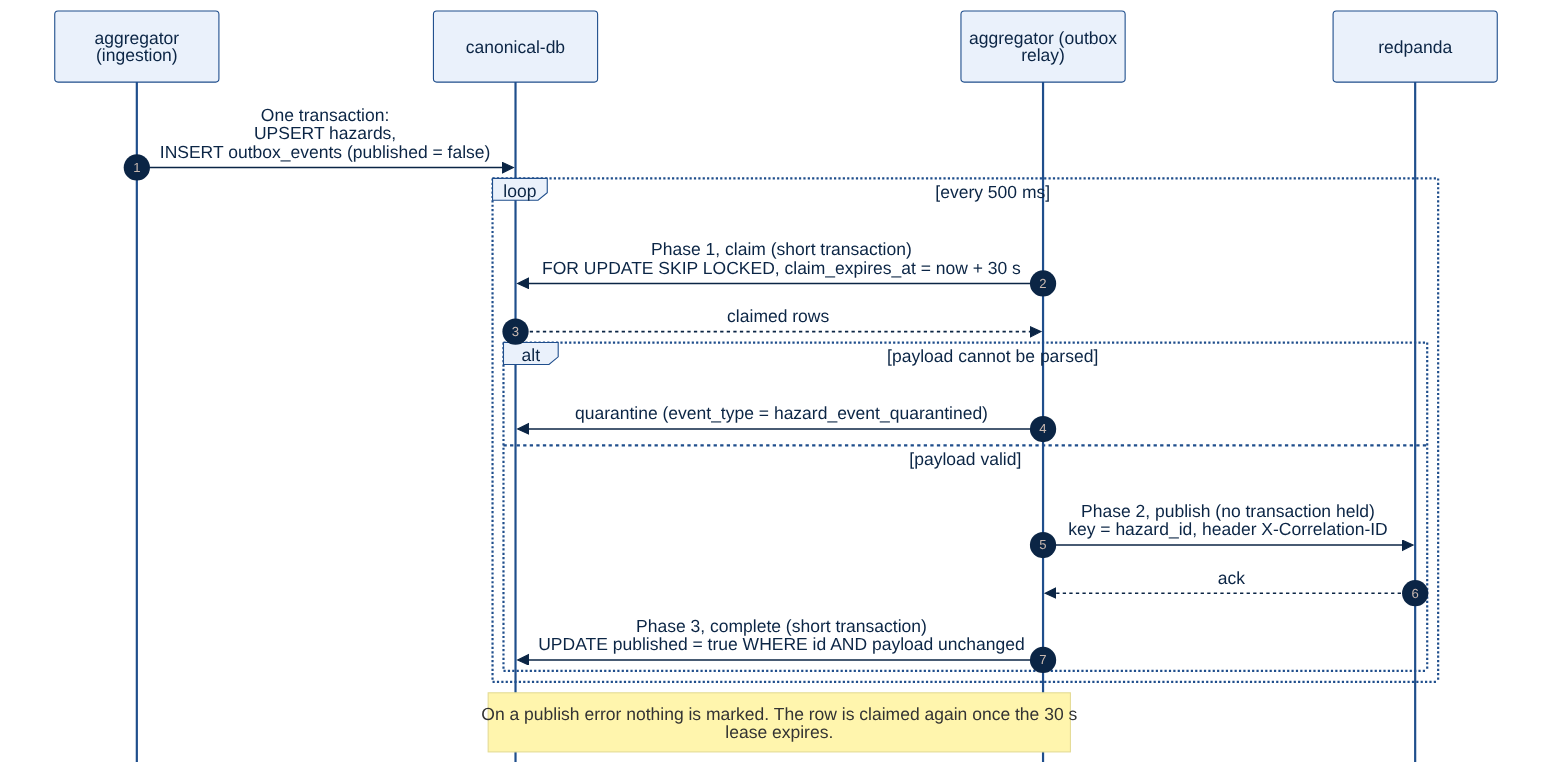
\includegraphics[width=\textwidth,height=0.55\textheight,keepaspectratio]{../diagrams/rendered/adr003-outbox.png}
    \caption[Tiga fase relay Transactional Outbox]{Tiga fase relay Transactional Outbox: claim, publish, dan complete (sumber: \texttt{adr003-outbox.mmd}).}
    \label{fig:relay_outbox}
\end{figure}

\clearpage
\subsection{Alasan Keputusan dan Trade-Off}
Tabel~\ref{tab:storage_eval} menyajikan perbandingan komparatif tiga opsi arsitektur penyimpanan:

\begin{table}[H]
\centering
\footnotesize
\begin{spacing}{1.05}
\caption{Evaluasi Komparatif Alternatif Arsitektur Penyimpanan}
\label{tab:storage_eval}
\begin{tabularx}{\textwidth}{p{2.8cm} X X X}
\toprule
\textbf{Kriteria} & \textbf{PostgreSQL + JSONB (Terpilih)} & \textbf{MongoDB (Document Store)} & \textbf{Strict SQL (EAV / Migrasi DDL)} \\
\midrule
Transaksionalitas \& Pola Outbox & \textbf{Sangat Kuat:} Mendukung transaksi ACID atomik antara tabel \texttt{hazards} dan \texttt{outbox\_events}. & \textbf{Kompleks:} Transaksi \mbox{multi-dokumen} memerlukan replica set (\texttt{--replSet} dan \texttt{rs.initiate()}) sebelum dapat dipakai. & \textbf{Kuat:} Mendukung transaksi ACID penuh. \\
\addlinespace
Agilitas Evolusi Skema & \textbf{Tinggi:} Atribut baru masuk ke JSONB tanpa \textit{table lock} atau migrasi DDL. & \textbf{Tinggi:} Skema dokumen secara alami dinamis. & \textbf{Rendah:} Memerlukan DDL \texttt{ALTER TABLE} atau tabel EAV yang rumit. \\
\addlinespace
Performa Query \& Indexing & \textbf{Tinggi:} Kolom relasional diindeks B-Tree standar; kolom JSONB dapat diindeks GIN. & \textbf{Sedang:} Kueri dokumen sangat cepat, namun tidak mendukung relasi JOIN. & \textbf{Sedang--Rendah:} Pola EAV memperlambat kueri karena banyaknya operasi JOIN. \\
\addlinespace
Kompleksitas Operasional & \textbf{Rendah:} Satu mesin basis data melayani kebutuhan relasional dan dokumen fleksibel. & \textbf{Sedang:} Menambah langkah inisialisasi replica set pada saat \textit{startup}. & \textbf{Rendah:} Mesin relasional tunggal namun beban migrasi skema tinggi. \\
\bottomrule
\end{tabularx}
\end{spacing}
\end{table}

\subsection{Batasan yang Disadari}
\begin{itemize}
    \item Kolom JSONB tidak menegakkan validasi tipe data pada level basis data. Integritas tipe nilai dalam atribut dinamis sepenuhnya menjadi tanggung jawab lapisan kode normalizer di Aggregator.
    \item Kueri berbasis teks bebas atau pencarian parsial di dalam dokumen \mbox{JSONB} yang belum diindeks GIN memerlukan \textit{full-table scan} parsial jika tabel bertumbuh hingga jutaan baris.
\end{itemize}

\subsection{Bukti Penyelesaian}
Verifikasi empiris diotomasi via target \texttt{make demo-p4} (\path{scripts/test_storage_restart.sh}) dengan rekaman log tersimpan pada berkas \path{docs/evidence/p4/storage_restart.log}:
\begin{enumerate}
    \item \textbf{Koeksistensi Skema Heterogen pada PostgreSQL (P4-02):}
    Kueri langsung ke basis data \texttt{canonical-db} membuktikan koeksistensi record sebelum dan setelah evolusi skema:

\noindent\begin{minipage}{\linewidth}
\begin{lstlisting}[language=SQL, caption={Hasil Kueri PostgreSQL Menunjukkan Koeksistensi Atribut Heterogen}]
-- Kueri LIMIT 3 pada tabel hazards (cuplikan, dipangkas)
-- BMKG  SEISMIC  WASPADA: {"depth_km": 37, "magnitude": 5, "potential_tsunami": false}
-- BMKG  SEISMIC  NORMAL : {"depth_km": 36, "magnitude": 4.9, "potential_tsunami": true}
-- PVMBG VOLCANIC WASPADA: {"volcano_id": "VLC-002", "confidence_level": 0.82,
--                          "eruption_count_24h": 8, "ash_column_height_m": 350}
\end{lstlisting}
\end{minipage}

    \item \textbf{Uji Restart Kontainer Independen (P4-01):}
    Kontainer \texttt{aggregator} dijalankan ulang (\textit{restart}) via Docker Compose. Selama proses berjalan, \texttt{client-api} (:8080) dan \textit{mock services} tetap merespons dengan HTTP 200 tanpa mengalami kegagalan berantai.
    \item \textbf{Pemulihan Mandiri Sambungan Basis Data:}
    Kontainer \texttt{canonical-db} dijalankan ulang (\textit{restart}). Klien API mendeteksi ketiadaan basis data sementara dan seketika pulih melayani permintaan dengan HTTP 200 begitu PostgreSQL siap menerima koneksi kembali.
\end{enumerate}

\subsection{Jawaban Butir Spesifikasi (Di Laporan)}
\textbf{Pertanyaan:} \textit{Jelaskan alasan penentuan batas tiap service, mengapa dipecah seperti itu dan bukan dengan pembagian lain. Serta, bandingkan minimal dua alternatif penyimpanan beserta konsekuensi dari pilihan yang diambil.}

\textbf{Jawaban:}
\begin{enumerate}
    \item \textbf{Alasan Penentuan Batas Service (\textit{Service Boundaries}):}
    Service dipecah berdasarkan batas domain dan tingkat perubahan (\textit{rate of change}):
    \begin{itemize}
        \item \textit{Aggregator} dipisahkan karena memiliki dependensi polling aktif dan merupakan satu-satunya penulis (\textit{single writer}) ke penyimpanan kanonis.
        \item \textit{Client-API} dipisahkan agar dapat diskalakan secara horizontal sesuai lonjakan lalu lintas baca publik tanpa membebani thread penarik data ke hulu.
        \item \textit{Auth Service} dipisahkan guna mengisolasi rahasia tanda tangan token kriptografi serta mencegah beban verifikasi autentikasi mengganggu pipa ingesti darurat.
    \end{itemize}
    \item \textbf{Perbandingan Alternatif Penyimpanan:}
    Dua alternatif utama dievaluasi (Tabel~\ref{tab:storage_eval}):
    \begin{itemize}
        \item \textit{Alternatif 1: Basis Data Dokumen Murni (MongoDB):} Keuntungannya fleksibel secara alami, namun konsekuensi buruknya adalah implementasi Transactional Outbox memerlukan transaksi \mbox{multi-dokumen}, yang pada MongoDB hanya tersedia pada replica set. Pengujian pada \texttt{mongo:7.0} menunjukkan mongod \textit{standalone} menolak transaksi, sedangkan replica set satu anggota sudah cukup, tetapi langkah \texttt{rs.initiate()} harus dijalankan lebih dahulu sebelum aplikasi dapat menulis (lihat ADR 003).
        \item \textit{Pilihan Terpilih: PostgreSQL 16 dengan Kolom JSONB:} Konsekuensinya adalah kelompok harus menjaga validasi skema atribut dinamis di lapisan aplikasi, namun memperoleh keuntungan besar berupa transaksi ACID tunggal atomik untuk outbox event, pengindeksan relasional yang matang, serta keandalan operasional tingkat tinggi.
    \end{itemize}
\end{enumerate}
